%!TEX root = paper.tex
\section{True Data Provenance}
\label{sec:provenance}

Provenance is powerful tool for {\em tracking} data artifacts. In the context of this paper, one might think of it as a way to identify the \emph{where} of the data error's story. Most practical and effective cleaning solutions follow a clean-and-evaluate lifecycle~\cite{Ilyas16DE}, which leverages the computational provenance of data analytics to track data errors to their sources, and attempts to provide explanations that lead to cleaning actions. This typical lifecycle is depicted in Figure~\ref{fig:lifecycle}. 
\begin{figure*}[ht]
  \centering
  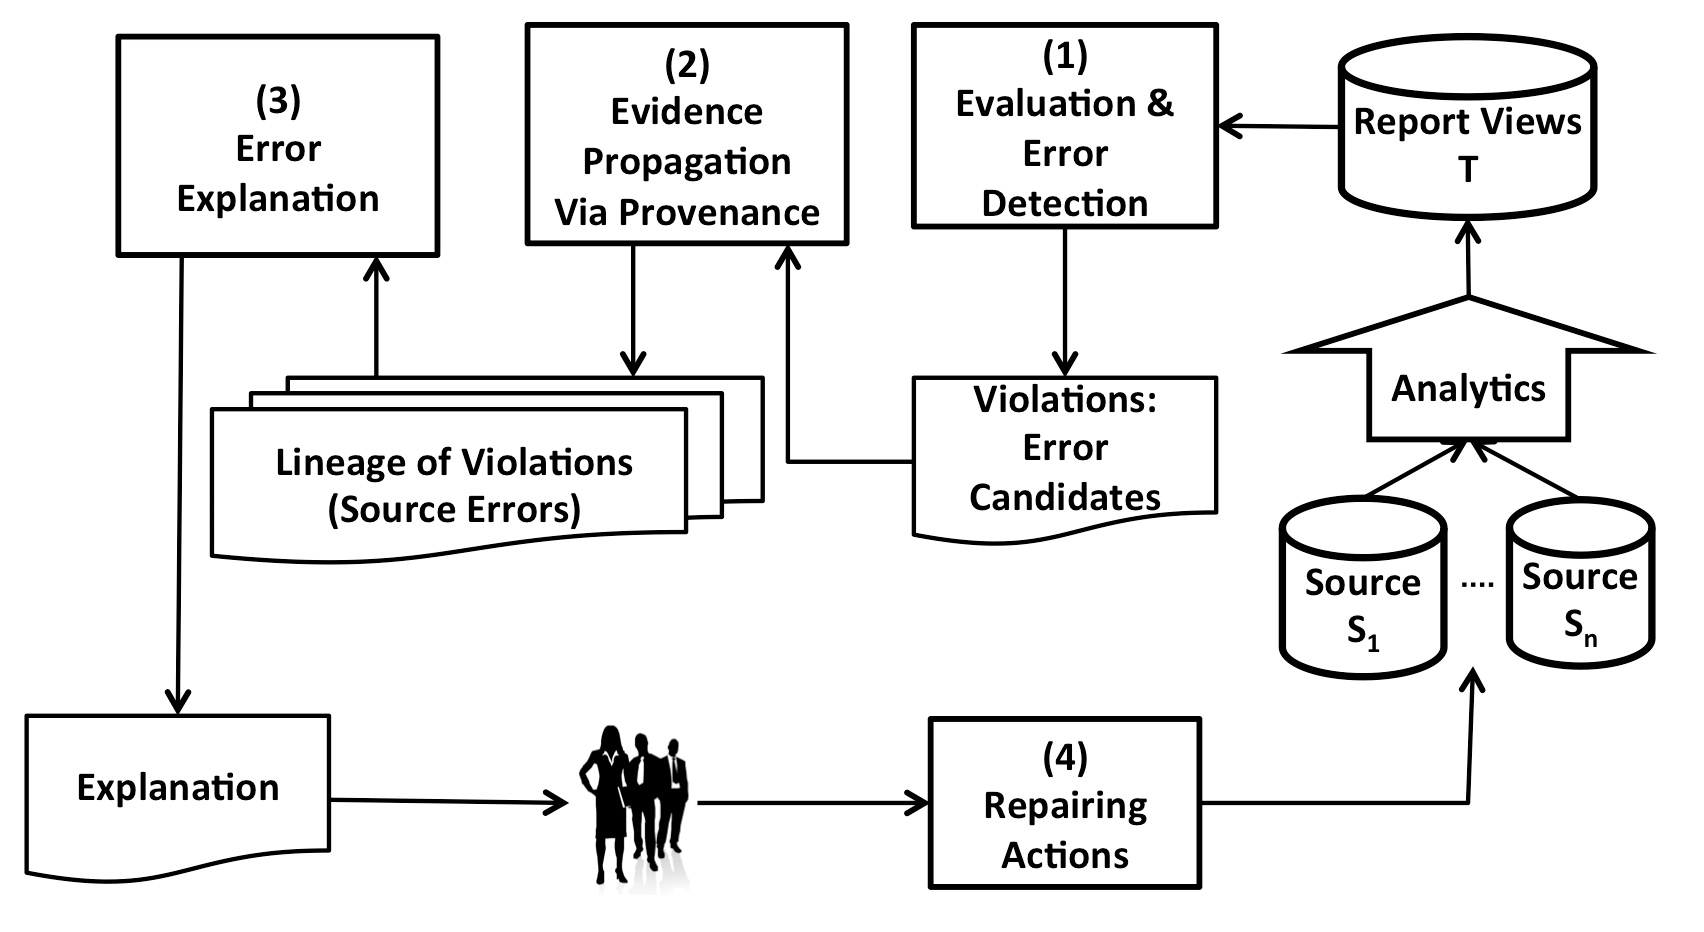
\includegraphics[width=0.6\textwidth]{lifecycle}
  \caption{Clean-and-Evaluate Loop~\cite{Ilyas16DE}}
  \label{fig:lifecycle}
\end{figure*}

Provenance and lineage systems focus on describing how the analytical {\em report views} are computed from the sources. For example, Scorpion~\cite{DBLP:journals/pvldb/0002M13}, DBRx~\cite{DBLP:conf/sigmod/ChalamallaIOP14} and QFix~\cite{DBLP:conf/sigmod/WangM017} (and many other followup work) are  solutions that trace back the tuples that contributed to the problems in the target to explain and help fix these errors at data sources. A recent survey summarizes the large body of work in debugging data-driven systems and explain what users see downstream from processing raw data~\cite{DBLP:journals/ftdb/GlavicMR21}. As these processing pipelines become more complex with cascades of large machine learning models, tracing errors in final predictions back to their causes can be very challenging. However, there is recent progress that can help us reason about observations in model predictions and track them back to errors in training data~\cite{DBLP:journals/corr/abs-2202-00622}.

The question becomes: \emph{is explaining errors in final analytics or predictions in terms of data sources enough?} What we refer to as ``raw data sources''  are often cut off the processes that generated these data, such as the human grader that input that data, the extraction script that generated this data from a webpage, or a presentation of the complex data pipeline that ran in a different software stack and generated this source data. From our discussions and involvement with large enterprises over the last decade, we argue that this decoupling is often due to two main reasons:
\begin{itemize}
\item \emph{Difficulty of integrating data processes in provenance systems:} Representing the process that generated the data might require expressive (and hence  complex) provenance systems. For example semiring-based  provenance systems have been extended  to capture information about external inputs (e.g., user choices), and  to capture process executions~\cite{DBLP:journals/vldb/DeutchMT15}; and in the context of scientific workflows,  the need for a control-flow driven workflow provenance model in contrast to the traditional  data-driven execution provenance paradigm has been explored~\cite{DBLP:journals/dke/ButtF21}.

\item \emph{Loss of provenance continuity across systems:}  We might be very careful in collecting and adequately presenting provenance information in the data pipelines we control. However, as the final data product (e.g., predictions, views, aggregates, or transformed data sets) get pushed to the downstream tasks, they are often treated as ``source data'' and downstream pipelines fail to  consume the associated provenance information.
\end{itemize}

Understandably, these are hard problems to tackle and part of the challenge is not even technical and it involves standardizing data provenance representation across business units and different software stacks. However, this might suggest new research directions; for example, we might prefer developing simpler and less expressive provenance models that target interoperability and ease of propagation over representation power of the underlying computations. Another example is that propagating standard meta-data that ties data sources to central data governance and catalogs can be part of the integrity constraints and sanity checks. We suggest also extending meta-data representation of data sources to include {\em repair actions} that reference a controlled vocabulary or a {\em repairing ontology} tapping into the large body of work in work flow and business processes management.




